\documentclass[../../General.tex]{subfiles}
\begin{document}


\section{Marco referencial}

En esta sección se detallan las normativas, las condiciones topográficas y el entorno operativo bajo los cuales funcionará el robot autónomo de medición.


\subsection{Contexto normativo y estándares de medición} 
Dado que el objetivo del vehículo es recolectar datos climáticos con validez industrial para el cálculo de índices de rendimiento, su instrumentación y métodos deben regirse estrictamente por la serie de estándares internacionales IEC 61724. Esta familia de normativas es la base para evaluar la capacidad y la energía de los sistemas fotovoltaicos. Dentro de esta serie, el principal referente para el diseño del hardware es la norma IEC 61724-1, la cual establece los requisitos para la monitorización del desempeño de sistemas fotovoltaicos y define las clases de exactitud exigidas para los sensores de irradiancia, temperatura y condiciones ambientales. Para topografías complejas, la norma subraya la necesidad de que los datos ambientales sean verdaderamente representativos de las condiciones que experimentan los módulos; de lo contrario, se genera una alta incertidumbre en el cálculo del \textit{Performance Ratio} \citep{IEC61724-1_2021}. Las exigencias de los parámetros más críticos definidos por esta norma, junto con su impacto en el proyecto, se detallan a continuación en la Tabla \ref{tab:requisitos_clase_ab}.




\begin{center}
\footnotesize
\begin{xltabular}{\textwidth}{|p{1.8cm}|>{\raggedright\arraybackslash}X|>{\raggedright\arraybackslash}X|p{2.8cm}|p{2.8cm}|}
\caption{Requisitos detallados por la Norma IEC 61724-1.}
\label{tab:requisitos_clase_ab} \\
\hline
\rowcolor[HTML]{D9E1F2} 
 &  &  & \multicolumn{2}{c|}{\textbf{Rango definido por la norma}} \\ \cline{4-5} 
\rowcolor[HTML]{D9E1F2} 
\multirow{-2}{*}{\textbf{Parámetro}} & \multirow{-2}{*}{\textbf{Descripción}} & \multirow{-2}{*}{\textbf{Impacto}} & \textbf{Clase A} & \textbf{Clase B} \\ \hline
\endfirsthead

\multicolumn{5}{c}%
{{\bfseries Continuación de la \tablename\ \thetable{}}} \\
\hline
\rowcolor[HTML]{D9E1F2} 
\textbf{Parámetro} & \textbf{Descripción} & \textbf{Impacto} & \textbf{Clase A} & \textbf{Clase B} \\ \hline
\endhead

\hline
\endfoot

\hline
\endlastfoot

\textbf{Clasificación} & Define las exigencias de exactitud y el diseño general para la recolección de datos. & Determina el rigor técnico y económico de la monitorización. & Alta exactitud (plantas grandes o a escala de red). & Exactitud media (instalaciones comerciales pequeñas o medianas). \\ \hline

\textbf{Intervalos} & Frecuencia de adquisición física (muestreo) y almacenamiento (registro). & Una alta frecuencia captura fluctuaciones rápidas y reduce la incertidumbre. & Muestreo máximo cada 5 segundos; Registro máximo cada 5 minutos, recomendado cada 1 minuto.. & Muestreo máximo cada 1 minuto; Registro máximo cada 5 minutos. \\ \hline

\textbf{Irradiancia} & Exigencias para los sensores de radiación incidente frontal y posterior. & Su exactitud define la incertidumbre final de la auditoría de rendimiento. & Piranómetro Clase A, espectralmente plano, incertidumbre menor al 2\%. & Piranómetro Clase C, incertidumbre menor al 3\%. \\ \hline

\textbf{Temperatura} & Medición térmica en la cara posterior del módulo y del aire circundante. & Dato vital para el cálculo de eficiencia corregido por temperatura. & \multicolumn{2}{p{5.6cm}|}{Resolución menor a $0,1^{\circ}\text{C}$ e incertidumbre entre $ \pm 1^{\circ}\text{C}$. El sensor de ambiente debe estar a 1 metro de distancia de fuentes térmicas.} \\ \hline

\textbf{Mitigación ambiental} & Protocolos de limpieza (\textit{soiling}) y sistemas contra rocío o escarcha. & Evita mediciones artificialmente bajas que afectarían el índice de rendimiento. & \multicolumn{2}{p{5.6cm}|}{Limpieza semanal o uso de tecnología automatizada de detección de \textit{soiling}} \\ \hline

\textbf{Distribución de sensores} & Muestreo espacial representativo de la irradiancia y temperatura en la planta. & Garantiza que los datos reflejen los microclimas y la topografía real del terreno. & \multicolumn{2}{p{5.6cm}|}{Requiere múltiples sensores distribuidos según la capacidad instalada.} \\ \hline

\textbf{Salida de planta} & Medidor principal de potencia y energía neta inyectada a la red. & Determina el cumplimiento de garantías y la facturación real. & Medidores de Clase 0.2 S. & Medidores de Clase 0.5 S. \\ \hline

\end{xltabular}
\end{center}

\subsection{Condiciones topográficas y geográficas}
Las plantas solares a gran escala se pueden instalar en terrenos irregulares y montañosos que presentan una topografía compleja, lo cual propicia la generación de microclimas y fluctuaciones espaciales en la radiación incidente. El diseño de la base móvil y el sistema de locomoción del robot están directamente condicionados por las severas exigencias de este entorno natural; como los desniveles pronunciados, que pueden alcanzar hasta los 15.8° \citep{Salinas2025}, como se puede observar en la Figura \ref{fig:PlantaPendiente}; o los obstáculos geológicos, que incluye maleza, arena suelta, rocas, zanjas profundas causas por erosión y charcos de lodo \citep{Figgis2025}. Estas complejas condiciones justifican la adopción de sistemas de tracción con alta adaptabilidad y agarre, como los sistemas de orugas, necesarios para superar áreas inestables.

\begin{figure}[H]
	% Fuerza la alineación izquierda y quita los ":" después del número
	\captionsetup{justification=raggedright, singlelinecheck=false, labelsep=none}
	
	\caption[Imagen aérea de varias colinas cubiertas con paneles fotovoltaicos en Jinhua, provincia de Zhejiang, China.]{} 
	
	\textit{Imagen aérea de varias colinas cubiertas con paneles fotovoltaicos en Jinhua, provincia de Zhejiang, China.} \par\medskip
	
	\centering
	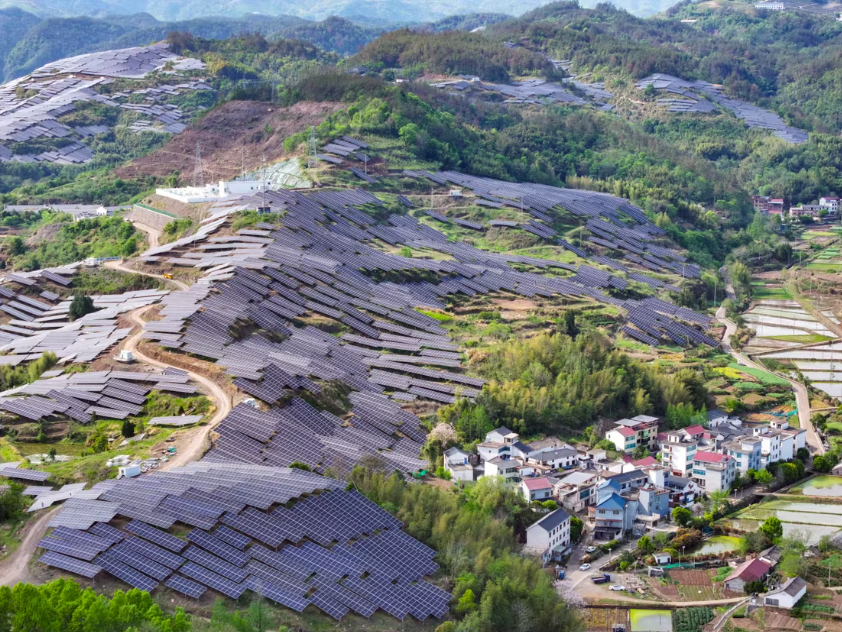
\includegraphics[width=0.6\textwidth]{Recursos/Imagenes/Otros/PlantaPendiente.png} \par\medskip
	
	\raggedright
	\footnotesize \textit{Nota.} Fotografía adaptada sobre la noticia ``China, the energy transition superpower''  \citep{Pouille2025China}.
	\label{fig:PlantaPendiente}
\end{figure}

\subsection{Entorno operativo y tecnológico}
El contexto operativo y tecnológico define las estrechas interacciones del vehículo autónomo con la infraestructura civil y electromecánica propia de la planta. El trazado de las instalaciones modernas se apoya mayoritariamente en estructuras con seguidores solares de un solo eje, orientados de norte a sur y separados por pasillos que oscilan entre los 5 y 9 metros de distancia \citep{ProyectoEjecutivo2024}.

En este escenario, la navegación autónoma del robot se verá restringida por obstáculos artificiales críticos. Entre ellos, la reducción del espacio transitable por la instalación de bandejas de distribución de cables y mallas reflectantes en el suelo, y la presencia de barras mecánicas entre las filas de los seguidores solares que impiden el libre tránsito transversal entre pasillos \citep{Figgis2025}. Todo ello exige que el robot disponga de un sistema de evitación de obstáculos robusto y una extrema precisión en su desplazamiento.

\end{document}